(by Vipin Singh)

\p
This chapter presents an analysis of the team structure essential for executing the business model.
It outlines the various roles within the organization and their contributions towards achieving the business objectives.
The focus lies on understanding the division of responsibilities and the collaborative efforts necessary for the company's growth and success.
This examination is intended to provide a clear view of the organizational framework and its significance in the operational realization of the business strategy.

\section{Team composition in the startup phase}
Since the business idea will start in a small scale, the human resources need to be used as efficiently as possible.
With only five founder members, this requires that each members role is not just defined by their job title.
Instead each member will have to be able to adapt and contribute across various facets of the business.
Still the business should also be able to scale up and expand its operations as it grows.

\p
With this said lets analyze the team composition, that is focused to rapidly develop and launch the product.

%TODO: Maybe create the table inline?
\begin{figure}[H]
    \centering
    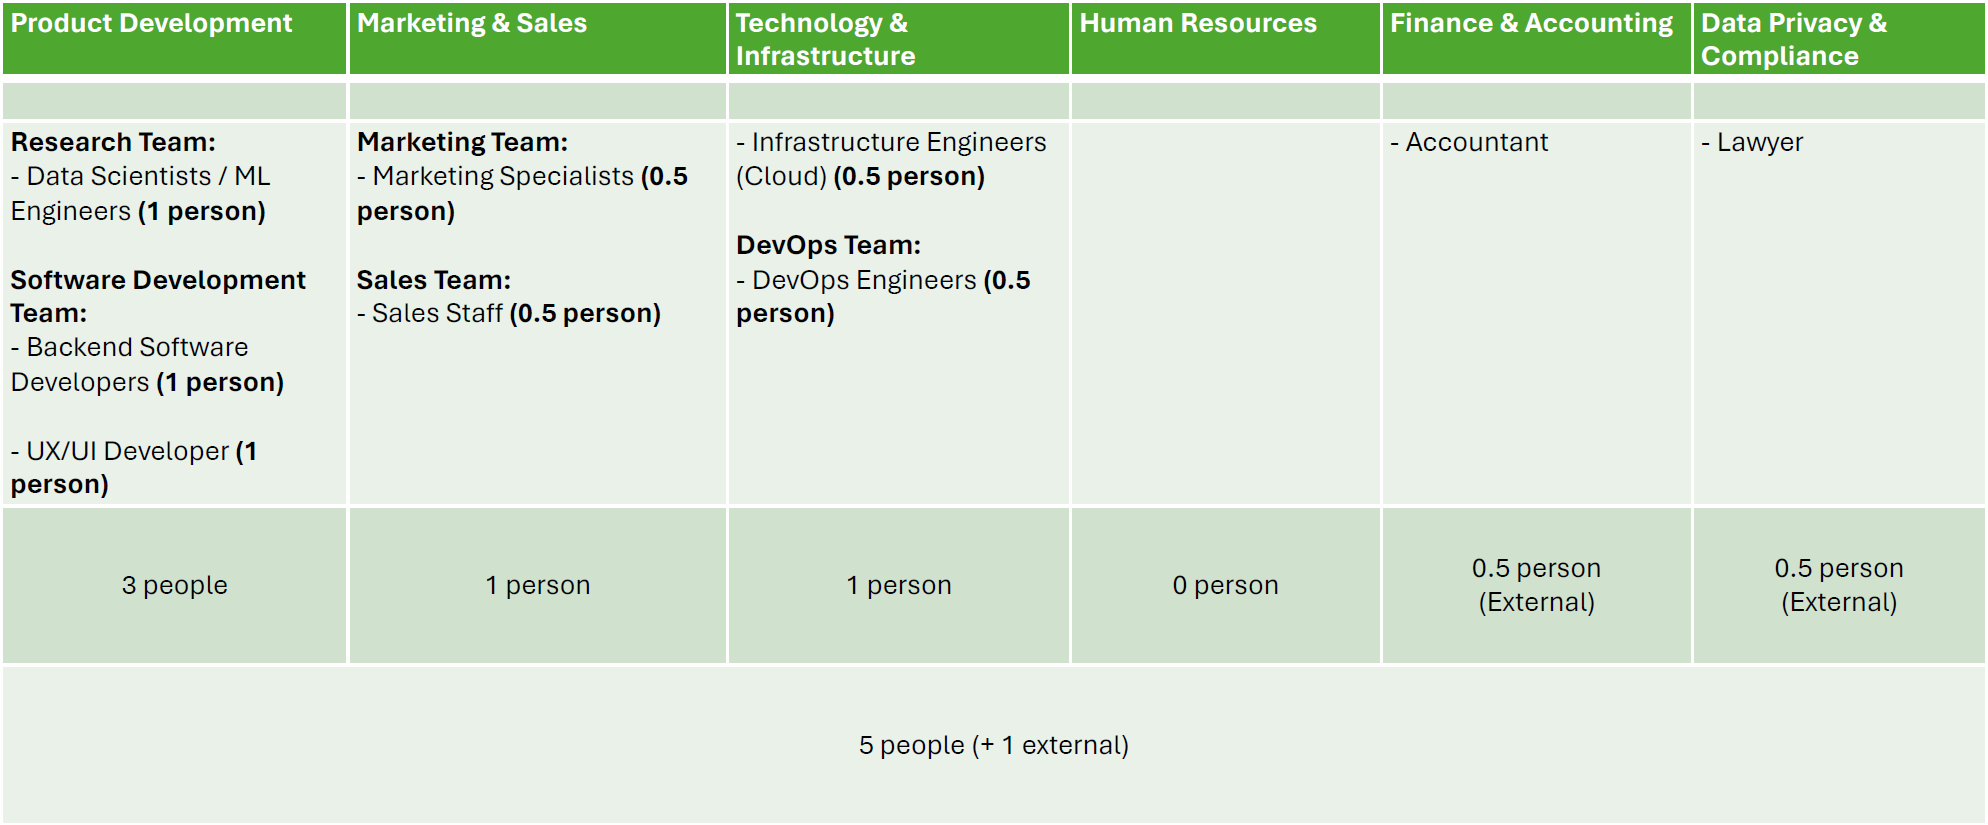
\includegraphics[width=\textwidth]{figures/team_comp_startup.png}
    \caption{Departments with team composition for a startup}
    \label{fig:team_comp_startup}
\end{figure}

In figure \ref{fig:team_comp_startup} we can see the team composition for a startup.
We decided to split the implementation of the team composition into six departments.
This department structure helps us to better understand the responsibilities we must fulfill for the business idea to succeed.
As we assign three out of the five founders to the product development department, it becomes clear that this is the core of our business for launching the product as fast as possible.

\p
Before we start with explaining the decisions for the team composition in figure \ref{fig:team_comp_startup}, we want to explain the responsibilities of each department and each role within the departments.

\subsection{Product Development}
The product development department serves as the core of innovation in our company.
It is responsible for designing the product by converting research insights into practical features.
It also ensures that the product is developed such that it meets the markets demand and holds the technical superiority over its competitors.
It is split into two teams, the Research team and the Software Development team.

\subsubsection*{Research Team}
The research team guides the development of new product features by providing insights into the latest research in the field of ergonomics and posture detection.
Therefore they are mainly responsible for the machine learning pipeline.
\begin{itemize}
    \item \textbf{Data Scientists / ML Engineers:}
            \begin{itemize}
                \item Keep track of foundation models for the task
                \item Analyze data to improve prediction accuracy for the posture keypoints
                \item Finetune the foundation models for our specific tasks with collected data
                \item Collaborate with software developers to integrate the machine learning pipeline into the product
            \end{itemize}
\end{itemize}

\subsubsection*{Software Development Team}
The software development team directly implements the product features into the codebase.
They also ensure that the product is scalable and maintainable, while having the user experience in mind.
Another important task that is not mentioned directly in the following is the testing of the products features and the documentation of the codebase.
\begin{itemize}
    \item \textbf{Backend Software Developers:}
            \begin{itemize}
                \item Write and maintain the codebase
                \item Implement new features
                \item Ensure scalability
            \end{itemize}
    \item \textbf{UX/UI Developer:}
            \begin{itemize}
                \item Design the user interface
                \item Design prototypes for new features
                \item Implement the designs for the user interface into the codebase
            \end{itemize}
\end{itemize}

\subsection{Marketing \& Sales}
The marketing and sales department functions as a crucial link between the product and the potential customers.
Its primary responsibilities are the development of marketing strategies that communicate the value proposition of the product to the target audience.
Furthermore they drive the sales initiatives to convert prospects into customers.
This is critical to generate revenue for the company.
The alignment of marketing and sales efforts ensure the customer acquisition and retention, which is vital for growth and success.
For further structure this department is split into two teams, the Marketing team and the Sales team.

\subsubsection*{Marketing Team}
\begin{itemize}
    \item \textbf{Marketing Specialists:} The marketing specialists are responsible for the marketing strategy and the marketing team.
\end{itemize}

\subsubsection*{Sales Team}
\begin{itemize}
    \item \textbf{Sales Staff:} The sales staff is responsible for the sales of the product.
\end{itemize}

\subsection{Technology \& Infrastructure}
The technology and infrastructure department is responsible for the technology and infrastructure of the product.
\begin{itemize}
    \item \textbf{IT Support Staff:} The IT support staff is responsible for the IT support of the product.
    \item \textbf{DevOps Engineers:} The DevOps engineers are responsible for the development and operation of the infrastructure of the product.
\end{itemize}

\subsection{Human Resources}
The human resources department is responsible for the human resources of the product.

\subsection{Finance \& Accounting}
The finance and accounting department is responsible for the finance and accounting of the product.
\begin{itemize}
    \item \textbf{Lawyer:} The lawyer is responsible for the legal aspects of the product.
\end{itemize}

\subsection{Data Privacy \& Compliance}
The data privacy and compliance department is responsible for the data privacy and compliance of the product.
\begin{itemize}
    \item \textbf{Accountant:} The accountant is responsible for the accounting of the product.
\end{itemize}

\section{Team composition after higher scaling}
\begin{figure}[H]
    \centering
    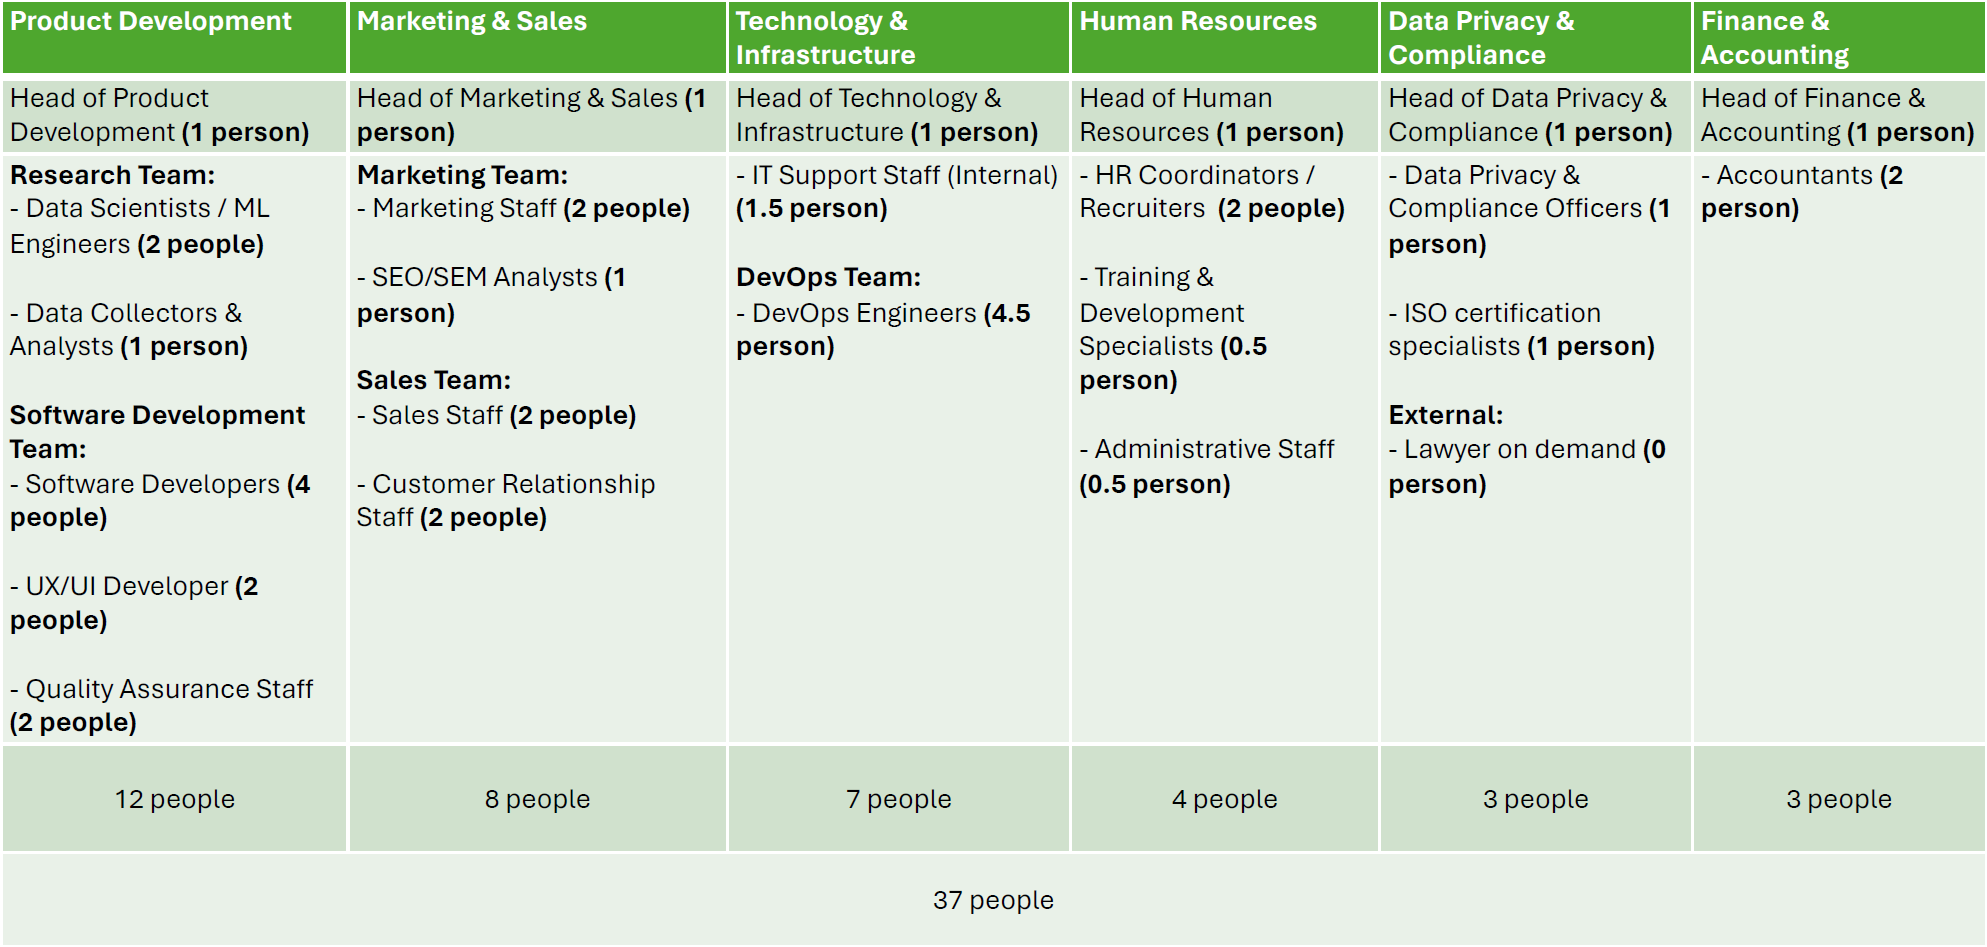
\includegraphics[width=\textwidth]{figures/team_comp_highscaled.png}
    \caption{Departments with team composition after the company has scaled up}
    \label{fig:team_comp_highscaled}
\end{figure}